% Credits : COLING 2018 style sheets
% Contact: zhu2048@gmail.com & liuzy@tsinghua.edu.cn
%% Based on the style files for COLING-2016, which were, in turn,
%% Based on the style files for COLING-2014, which were, in turn,
%% Based on the style files for ACL-2014, which were, in turn,
%% Based on the style files for ACL-2013, which were, in turn,
%% Based on the style files for ACL-2012, which were, in turn,
%% based on the style files for ACL-2011, which were, in turn, 
%% based on the style files for ACL-2010, which were, in turn, 
%% based on the style files for ACL-IJCNLP-2009, which were, in turn,
%% based on the style files for EACL-2009 and IJCNLP-2008...

%% Based on the style files for EACL 2006 by 
%%e.agirre@ehu.es or Sergi.Balari@uab.es
%% and that of ACL 08 by Joakim Nivre and Noah Smith
\documentclass[11pt,francais]{article}
\usepackage{coling2018}
\usepackage[utf8]{inputenc} 
\usepackage[T1]{fontenc}
\usepackage{babel} 
\usepackage{times}
\usepackage{url}
\usepackage{latexsym}
\usepackage{xcolor}
\usepackage{graphicx}
\usepackage{todonotes}
\usepackage{verbatim}

\usepackage{amssymb}
\usepackage{hyperref}       % hyperlinks
\usepackage{subcaption}
\usepackage{appendix}
\usepackage[export]{adjustbox}

\title{Rapport de stage : GAN}

\author{Lucas Goareguer \\
  Aix-Marseille Université \\
  {\small \texttt{Lucas.Goareguer@etu.univ-amu.fr}   } \\\And
   {\bf Supervision : Laurent Perrinet} \\
  Institut de Neurosciences de la Timone \\
  {\small \tt Laurent.Perrinet@univ-amu.fr} \\}
\date{}

%%%%%%%%%%%%%%%%%%%%%%%%%%%%%

\begin{document}
\maketitle
\begin{abstract}
Ce papier à pour objectif de décrire le travail effectuer durant le stage final du Master Intelligence Artificielle et Apprentissage Automatique.
Ce stage de 6 mois c'est dérouler à l'Institut de Neurosciences de la Timone et a était encadrer par Laurent Perrinet, enseignant chercheur à l'université d'Aix-Marseille.
Le principal objectif du stage était la compréhension des Generative Adverserials Networks (GAN) appliquer à la génération d'images. Un des apports important de ce travail à était le développement d'outils facilitant la création de GANs, notamment une librairies consacrer a cette tâche ainsi qu'un outils de scan des hyper-paramètres.
\end{abstract}

\blfootnote{
This work is licensed under a Creative Commons 
Attribution 4.0 International License.
License details:  \url{http://creativecommons.org/licenses/by/4.0/}}

%%%%%%%%%%%%%%%%%%%%%%%%%%%%%
\section{Motivation}

\subsection{Pourquoi les GANs}
\label{sec:Intro}
% https://stackoverflow.com/questions/50131068/producing-stacked-3d-blocks-using-tikz
Les réseaux génératifs adversaires ou Generatif Adverserial Networks (GAN) en anglais sont des modèles qui permettent, par un apprentissage non superviser, de générer des données cohérentes par rapport a un dataset donnée. Ils on était décrit pour la première fois en 2014 dans l'article de I. Goodfellow \cite{NIPS2014_5423}, depuis ils on connus un intérêt grandissant et de nombreux chercheur s'y sont intéresser comme en témoignent cette page référençant de nombreux article : \href{https://github.com/hindupuravinash/the-gan-zoo}{The Gan Zoo} \footnote{\label{note1}The Gan Zoo : https://github.com/hindupuravinash/the-gan-zoo}.\\
L'usage des GANs comme un outils de compréhension de notre cerveau est tentant en neurosciences. Le pas a notamment était franchie concernant le parallèle entre imagination et modèles génératifs via les travaux de \cite{GAN_Brain_Signals} qui tendent notamment à montrer un lien entre la façon dont les images sont générer dans notre cerveaux et dans les GANs. 
Cette technologie étant très intéressante à bien des égards la tâche qui ma était confier lors de mon stage à était d'étudier les GANs et de développer des outils permettant de les utilisées et de les paramétrées. 

\subsection{Generatif Adverserial Networks (GAN)}
\label{sec:GAN}
\begin{figure}[!b]
    \centering
    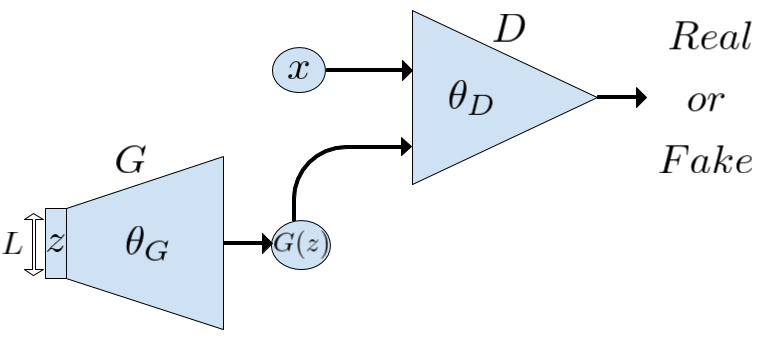
\includegraphics[width=\textwidth]{Figures/GAN/GAN_representation.png}
    \caption{Architecture d'un GAN.}
    \label{fig:fig9}
\end{figure}
Les réseaux génératifs adversaires (GAN) sont des modèles qui permettent de générer des données approchant une lois de probabilités cible \(P\) données par un dataset.
Ces modèles dans la version d'origine présenter par I. Goodfellow \cite{NIPS2014_5423} ce présente sous la forme de deux réseaux distinct : \\
  - Un générateur \(G\) qui prend en entrée un vecteur aléatoire \(z\) dans un l'espace latent de taille \(L\) et produit en sortie une donnée qui, après un entraînement réussi, doit être cohérente par rapport à \(P\). Les poids de \(G\) sont notés \(\theta_G\) (c.f. figure \ref{fig:fig9}) ;\\
  - Un discriminateur \(D\) qui a pour objectif de déterminer si les données qui lui sont présenter en entrée suive la loi de probabilité \(P\) ou non. Autrement dit si elle appartiennent au dataset ou non.
  Les poids de \(D\) sont notés \(\theta_D\) (c.f. figure \ref{fig:fig9}) .\\
Ces deux réseaux vont être entraîner en parallèles par backpropagation en minimisant les fonctions de pertes suivantes pour chacun des deux réseaux.\\
\(lossD = -log(D(x)) - log(1-D(G(z))) \) \\
\(lossG = -log(D(G(z))) \) \\
Avec x les données du dataset.\\
Ces deux losses ce rapportes dans notre cas à la fonction de Binary Cross Entropy t-elle que : 
\[
BCE(x, y) = -[y * log(x) + (1 - y) * log(1 - x)]
\]
Avec x les réponse données par \(D\) pour des images et y les réponse attendues pour ces images.

Pour entrainer les deux réseaux on suis l'algorithme suivant :
\begin{table}[hb]
  \begin{tabular}{l}
  \hline
  Algorithme 1: Entraînement d'un GAN\tabularnewline
  \hline
  Entrées: Nombre d'itération de l'entraînement  \(I\), la taille des batchs \(B\), le dataset \(data\)  \tabularnewline
  Sortie: G, un générateur entraîner \tabularnewline
  \hline
  Pour \(I\) étapes faire :\tabularnewline 
  \hspace{1cm}\(z \leftarrow\) ensemble de \(B\) vecteur de taille \(L\) \(\sim \mathcal{N}(0,1)\);\tabularnewline
  \hspace{1cm}\(imagesGenerees \leftarrow\) \(G(z)\);\tabularnewline  
  \hspace{1cm}\(imagesReels \leftarrow\) échantillons de \(B\) images de \(data\);\tabularnewline
  \hspace{1cm}\(Fake \leftarrow\) vecteur de taille \(B\) remplie de 0;\tabularnewline
  \hspace{1cm}\(Valid \leftarrow\) vecteur de taille \(B\) remplie de 1;\tabularnewline
  \tabularnewline
  \hspace{1cm}// Entraînement de D\tabularnewline
  \hspace{1cm}\(d_x \leftarrow D(imagesReels)\);\tabularnewline
  \hspace{1cm}\(d_{g_z} \leftarrow D(imagesGenerees)\);\tabularnewline
  \hspace{1cm}\(lossD \leftarrow BCE(d_x,Valid) + BCE(d_{g_z},Fake)\);\tabularnewline
  \hspace{1cm}Utilisation de \(lossD\) pour mettre à jour \(\theta_D\) par descente de gradient stochastique;\tabularnewline
  \tabularnewline
  \hspace{1cm}// Entraînement de G\tabularnewline
  \hspace{1cm}\(lossG\leftarrow BCE(d_{g_z},Valid)\);\tabularnewline
  \hspace{1cm}Utilisation de \(lossG\) pour mettre à jour \(\theta_G\) par descente de gradient stochastique;\tabularnewline
  \tabularnewline
  return G;\tabularnewline
  \hline
  \end{tabular}
  \label{tab:tab1}
\end{table}

L'algorithme utiliser pour effectuer les descentes de gradient lors de nos expériences est \href{https://arxiv.org/pdf/1412.6980.pdf}{ADAM} \cite{kingma2014adam}.\\
L'entraînement est arrêter lorsque le nombres d'étapes choisi est atteint hors les images générer par G ne sont pas forcement cohérente au yeux de l'observateur. C'est l'un des problèmes qui entoure les GANs et que nous allons introduire dans la section suivantes.

\subsection{Compréhension des limites théoriques de ces modèles}
\label{sec:CompEtLimites}
Une part importantes de nos recherche on consister a essayer de comprendre les barrières théorique qui entoure les GANs et leurs apprentissage.
Les difficultés rencontrer lors de l'apprentissage d'un GANs sont importante notamment à cause de la difficultés qu'il y à a mesurer la qualité de l'apprentissage durant l'entraînent. En effet aucune mesure ne permet directement de savoir si les images générer sont cohérente au vus du dataset. L'objectif pratique des GAN n'est pas d'obtenir un générateur qui produisent exactement les images du dataset mais plutot de produire des images à la fois diverses et proches des données. C'est cette notion de distance entre les images générer et celles du dataset qui est difficiles a mesurer et c'est pourquoi la plupart du temps il est nécessaire d'observer les images générer pour jugée de la qualité de l'entraînement.\\
Nous nous sommes également pencher sur le problème dit de "mode collapse" (effondrement du mode en anglais) qui fait référence a un apprentissage lors du quel le générateur ce mets à produire des images peut diversifier et souvent incohérente compte tenus du dataset. Ce problème a notament était étudier dans la section 3.2 de \cite{salimans2016improved} et dans la section 2.4 de \cite{DBLP:journals/corr/MetzPPS16}.
Ces questions seront discutée dans la section \ref{sec:LossG_et_Convergeance}.

\subsection{Adverserial Auto-Encoder (AAE)}
\label{sec:AAE}
\begin{figure}[!h]
    \centering
    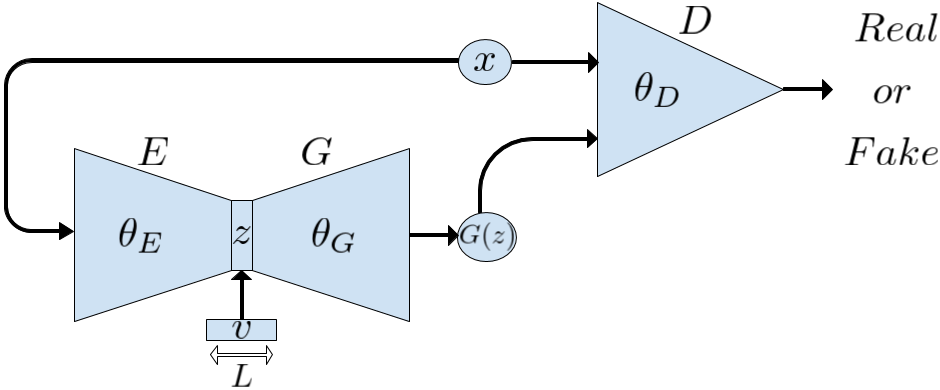
\includegraphics[width=\textwidth]{Figures/GAN/AAE_representation.png}
    \caption{Architecture d'un AAE. Le vecteur \(v\) représente une entrée direct de \(G\) sans passer par \(E\).}
    \label{fig:fig10}
\end{figure}

% http://www.texample.net/tikz/examples/simple-flow-chart/
On trouve dans la littérature différentes formes d'auto-encoder adversaires, comme par exemples cette version qui est la plus répandue \cite{makhzani2015adversarial}.
Pour les expériences sur l'étude des espaces latent que nous détailleront par la suite nous avons choisis d'utiliser une architecture proche de celle présenter dans l'article \cite{GADAE}.
Dans ce modèles on trouve dans un premier temps un auto-encoder standard avec un goulot d'étranglement, ou espace latent de faible dimension \(L\), au centre et à l'entrée un encoder \(E\), avec pour poids \(\theta_E\), charger de réduire la dimension des données et en sortie un décoder \(G\) charger d'augmenter la dimension du vecteur latent jusqu'à la taille des données et qui sert également de générateur. On associe ce réseau à un discriminateur \(D\) charger de déterminer si les images qui lui sont présenter viennent du décoder ou du dataset.

Les fonctions de pertes utiliser pour entraîner ce réseaux sont :
\[
lossD = -log(D(x)) - log(1-D(G(z)))
\]
\[
lossG = -log(D(G(z)))
\]
\[
lossEG = MSE(x, G(E(x))) + MSE(z_{imgs}, z_{zeros}) + MSE(z_{imgs}^2, z_{ones})^{0.5}
\]
Avec MSE définie comme l'erreur quadratique moyenne.
Le \(lossEG\) sera détaillais dans la sous section suivante \ref{sec:LatentSpace}.

On suis un algorithme d'entraînement légèrement diffèrent que pour les GANs standard que voici :\\
\begin{table}[!h]
  \begin{tabular}{l}
  \hline
  Algorithme 2: Entraînement d'un AAE\tabularnewline
  \hline
  Entrées: Nombre d'itération de l'entraînement  \(I\), la taille des batchs \(B\), le dataset \(data\)  \tabularnewline
  Sortie: G, un générateur entraîner \tabularnewline
  \hline
  Pour \(I\) étapes faire :\tabularnewline 
  \hspace{1cm}\(z \leftarrow\) ensemble de \(B\) vecteur de taille \(L\) \(\sim \mathcal{N}(0,1)\);\tabularnewline
  \hspace{1cm}\(imagesGenerees \leftarrow\) \(G(z)\);\tabularnewline  
  \hspace{1cm}\(imagesReels \leftarrow\) échantillons aléatoire de \(B\) images de \(data\);\tabularnewline
  \hspace{1cm}\(Fake \leftarrow\) vecteur de taille \(B\) remplie de 0;\tabularnewline
  \hspace{1cm}\(Valid \leftarrow\) vecteur de taille \(B\) remplie de 1;\tabularnewline
  \tabularnewline
  
  \hspace{1cm}// Entraînement de EG\tabularnewline
  \hspace{1cm}\(z_{zeros} \leftarrow\) ensemble de \(B\) vecteur de taille \(L\) remplie de 0;\tabularnewline
  \hspace{1cm}\(z_{ones} \leftarrow\) ensemble de \(B\) vecteur de taille \(L\) remplie de 1;\tabularnewline
  \hspace{1cm}\(z_{imgs} \leftarrow E(imagesReels)\);\tabularnewline
  \hspace{1cm}\(decoded_{imgs} \leftarrow G(z_{imgs})\);\tabularnewline
  \hspace{1cm}\(lossEG \leftarrow MSE(imagesReels, decoded_{imgs}) + MSE(z_{imgs}, z_{zeros}) +\)\tabularnewline
  \hspace{2,8cm}\(MSE(z_{imgs}^2, z_{ones})^{0.5}\);\tabularnewline
  \hspace{1cm}Utilisation de \(lossEG\) pour mettre à jour \(\theta_E\) et \(\theta_G\) par descente de gradient stochastique;\tabularnewline
  \tabularnewline
  
  \hspace{1cm}// Entraînement de D\tabularnewline
  \hspace{1cm}\(d_x \leftarrow D(imagesReels)\);\tabularnewline
  \hspace{1cm}\(d_{g_z} \leftarrow D(imagesGenerees)\);\tabularnewline
  \hspace{1cm}\(lossD \leftarrow BCE(d_x,Valid) + BCE(d_{g_z},Fake)\);\tabularnewline
  \hspace{1cm}Utilisation de \(lossD\) pour mettre à jour \(\theta_D\) par descente de gradient stochastique;\tabularnewline
  \tabularnewline
  
  \hspace{1cm}// Entraînement de G\tabularnewline
  \hspace{1cm}\(lossG\leftarrow BCE(d_{g_z},Valid)\);\tabularnewline
  \hspace{1cm}Utilisation de \(lossG\) pour mettre à jour \(\theta_G\) par descente de gradient stochastique;\tabularnewline
  \tabularnewline
  
  return G;\tabularnewline
  \hline
  \end{tabular}
  \label{tab:tab2}
\end{table}

L'intérêt d'un telle dispositif est qu'il permet d'avoir un accès direct à l'espace latent. Ainsi on pourras par la suite mener des expériences sur la façon dont est construit l'espace latent.

\subsection{Étude de l'espace latent et lossEG}
\label{sec:LatentSpace}
%lien avec VAE de Kingma \url{https://arxiv.org/pdf/1312.6114.pdf}
Le \(lossEG\) est, comme vous l'aurez sûrement remarquer, un peut particuliers. Il s'inspire d'un article de Kingma \cite{kingma2013auto} dans lequel est détailler une méthodes permettant notamment de contraindre une loi de probabilités quelconques à suivre une loi Gaussienne.
L'idée ici est de faire en sorte que l'espace latent de l'auto-encoder (et donc celui du générateur) soit contraint à une loi Gaussienne ainsi les vecteurs \(z\) associé au images du dataset seront plonger dans un espace latent contrôlée et que l'on pourras faire correspondre avec celui des images générer aléatoirement.  En créant cette correspondance entre les deux espaces latents on pourras les étudiées en détails ce qui sera le sujet de l'une des expériences que nous présentons dans la section \ref{sec:CorrespondancesLS}.

%%%%%%%%%%%%%%%%%%%%%%%%%%%%%
\section{Méthodes}

\subsection{Scan des paramètres}
\label{sec:ParamsScans}
Le nombre important d'hyper-paramètres présent dans les GANs nous a pousser à développer un outils permettant de passer en revus un nombre important de paramètres pour un GANs donnée. Ainsi nous avons peut parcourir de manières efficace ces immenses espace de paramètres.
Nous avons par la suite très largement utiliser cet outils pour réglé nos GANs durant toutes les expériences qui seront décrite par la suite. 

\subsection{Simpsons Dataset}
\label{sec:SimpsonsDataset}

\begin{figure}[!h]
    \centering
    \begin{subfigure}[b]{0.19\textwidth}
        
\includegraphics[width=\textwidth]{Figures/Simpsons_Dataset/13.png}
    \end{subfigure}
    \begin{subfigure}[b]{0.19\textwidth}
        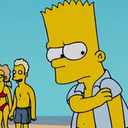
\includegraphics[width=\textwidth]{Figures/Simpsons_Dataset/15.png}
    \end{subfigure}
    \begin{subfigure}[b]{0.19\textwidth}
        
\includegraphics[width=\textwidth]{Figures/Simpsons_Dataset/25.png}
    \end{subfigure}
    \begin{subfigure}[b]{0.19\textwidth}
        
\includegraphics[width=\textwidth]{Figures/Simpsons_Dataset/8.png}
    \end{subfigure}
    \begin{subfigure}[b]{0.19\textwidth}
        
\includegraphics[width=\textwidth]{Figures/Simpsons_Dataset/18.png}
    \end{subfigure}
    \caption{Exemples d'images du dataset Simpsons Faces utiliser pour certaine expériences.}
    \label{fig:fig1}
\end{figure}

Pour certaine de nos expériences nous avons utiliser le dataset \href{https://www.kaggle.com/kostastokis/simpsons-faces}{Simpsons Faces} \footnote{\label{note2}Simpsons Faces : https://www.kaggle.com/kostastokis/simpsons-faces}. Ce dataset contient 9877 images de visage des personnages des Simpsons extrait des épisodes de manières automatique. Ce processus  automatique à introduit un certain nombres d'erreur dans les données (aucun personnages sur l'images, des visages couper, ect...), pour cette raison j'ai effectuer une passe manuel pour retirer au maximum ces mauvaise image du dataset et nous avons finalement utiliser 9629 images pour nos expériences. Vous pouvez voir quelques exemples d'images de ce dataset sur la figure \ref{fig:fig1}.\\
Nous avons choisi d'utiliser ces images en taille 128 par 128 pixels pour nos expériences.

\subsection{Simpsons Generator}
\label{sec:SimpsonsGenerator}
La première partie du stage à consister en une exploration du monde des GANs. Nous nous somme donc fixé comme objectif la rechercher, l'étude et l'entraînement d'un modèle capable de générer des visages de personnages des Simpson.
Après avoir choisi le sujet de nos expériences nous avons explorer l'immense monde des GANs et nous avons rapidement dû faire des choix étant données la quantité astronomique d'article présentant des variantes de GAN (c.f. \href{https://github.com/hindupuravinash/the-gan-zoo}{The Gan Zoo} \ref{note1}).
Nous avons donc focaliser notre attention sur les systèmes les plus éprouver afin de comprendre au mieux la théorie derrières ces modèles.\\
Nous avons particulièrement utiliser les DCGAN \cite{radford2015unsupervised} qui sont notamment composer de couches de convolution très adapter au traitement des images. Puis dans un second temps nous nous sommes pencher sur les Adverserial Auto-Encoders (AAE)  qui nous on servie par la suite pour l'expérience présenter en section \ref{sec:CorrespondancesLS}.

\subsection{Fractal Dream Dataset}
\label{sec:FDD}
\begin{figure}[!h]
    \centering
    \begin{subfigure}[b]{0.20\textwidth}
        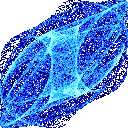
\includegraphics[width=\textwidth]{Figures/FDD/-0,00545687187361743_-0,5312304575586382_1,8197494653032407_2,422111729355857_1,4944898296889655_2,487490210145214.png}
    \end{subfigure}
    \begin{subfigure}[b]{0.20\textwidth}
        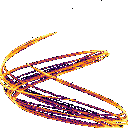
\includegraphics[width=\textwidth]{Figures/FDD/-0,319459804135373_-0,0981842500805612_0,42291442353441633_1,7253282321258185_1,4272325555244099_1,3701336149016234.png}
    \end{subfigure}
    \begin{subfigure}[b]{0.20\textwidth}
        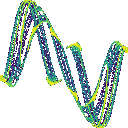
\includegraphics[width=\textwidth]{Figures/FDD/-0,9333646250089_-0,3698044331245828_-1,9514116449042127_-0,376713271698188_-1,1759178511809651_-1,7157801385982319.png}
    \end{subfigure}
    \caption{Exemples d'images du dataset Fractal Dream Dataset utiliser pour certaine expériences. Vous pourrez trouver la liste des paramètres utiliser pour générer ces trois figures en annexes \ref{appendix:annexe1}}
    \label{fig:fig2}
\end{figure}

Pour l'une des expériences que nous souhaitions mener (c.f. section \ref{sec:CorrespondancesLS}), nous avions besoin d'un dataset particulier.
En effet il nous fallait un dataset dont chaque images puisse être associer à un point dans l'espace de manière cohérentes.
Pour ce faire nous avons décider de construire un nouveau dataset à partir d'un outils mathématique : les attracteur étrange \cite{Pickover}. Ces objets permettent notamment de générer des figures varier à partir d'un nombre donnée de paramètres.
Les Fractal Dream \cite{Pickover} sont un type particuliers d'attracteur étrange que nous avons choisi pour notre dataset. A partir de 6 paramètres, la formule disponibles en annexes \ref{appendix:annexe1} permet de calculer de manière itérative (pour un nombre d'itération donner) un ensemble de points qui constitue la trajectoire de l'attracteur et qui placer dans un quadrillage de taille fini (128 par 128 dans notre cas) donne une images comme celles visibles dans la figure \ref{fig:fig2}. Dans les images les nuances de couleurs des pixels correspondes aux nombres de fois ou l'attracteur est passer dans la case.
Le dataset est constituer de trois classes d'images correspondant aux trois palettes de couleurs choisi (bleu, orange et vert), pour nos expériences nous n'avons utiliser qu'une seul de ces trois palettes pour faciliter l'entraînement.
Le dataset construit pour l'occasion ainsi que les codes utiliser on était mis à disposition sur le site Kaggle (ref).

\subsection{Correspondances des espaces latent}
\label{sec:CorrespondancesLS}
La façon dont est construit l'espace latent du générateur des GANs nous à fait nous poser de nombreuse questions.
Nous avons notamment voulus savoir si étant donnée un dataset \(data\) composer d'images \(x\), chacune associer à un unique vecteur \(v\), de dimension \(L\), répartie de manière cohérente dans l'espace. Un générateur \(G\) entraîner avec un AAE (comme décris dans la section \ref{sec:AAE}), pourrait-il générer une image \(x'\) proche de celle d'un \(x\) pris au hasard dans \(data\) pour un même vecteur \(v\). Autrement dit : le générateur serait-il capable de reconstruire par un entraînement adversaire la cohérence qui relis les images de \(data\) au vecteur \(v\) qui leurs est associer. 
Pour mettre en place cette expériences nous avons entraîner un AAE avec le dataset FDD présenter dans la section \ref{sec:FDD}. Ensuite nous avons pu comparer les images de FDD au images générer par \(G\) pour un même vecteur \(v\).

\begin{figure}[!h]
    \centering
    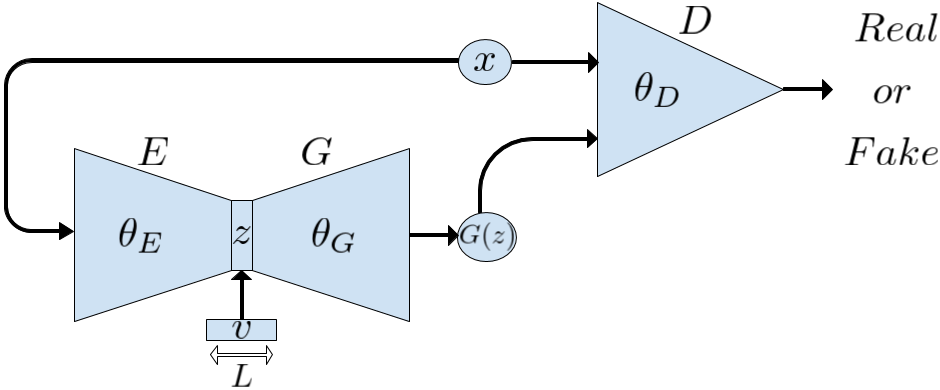
\includegraphics[width=\textwidth]{Figures/GAN/AAE_representation.png}
    \caption{Architecture d'un AAE. Le vecteur \(v\) représente une entrée direct de \(G\) sans passer par \(E\).}
    \label{fig:fig10}
\end{figure}


%%%%%%%%%%%%%%%%%%%%%%%%%%%%%
\section{Résultats}

\subsection{Simpsons Cohérent}
\label{sec:SimpsonsCoherent}
\begin{figure}[!h]
    \centering
    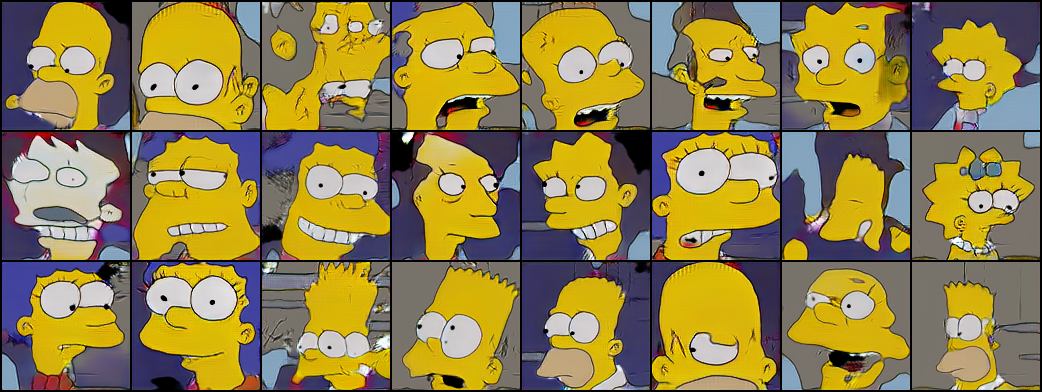
\includegraphics[width=\textwidth]{Figures/resultats_simpsons/DCGAN_270.png}
    \caption{Images générer avec le générateur d'un DCGAN après 270 epochs d'entraînement.}
    \label{fig:fig3}
\end{figure}

\begin{figure}[!h]
    \centering
    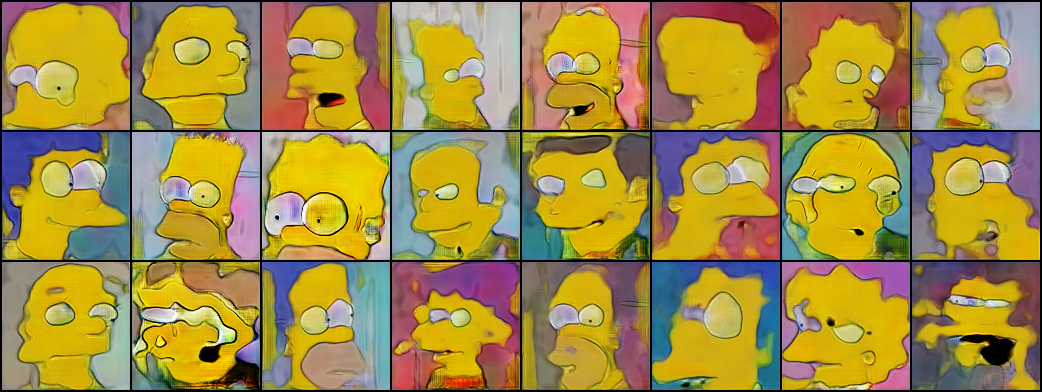
\includegraphics[width=\textwidth]{Figures/resultats_simpsons/AAE_300.png}
    \caption{Images générer avec le générateur d'un AAE après 300 epochs d'entraînement.}
    \label{fig:fig4}
\end{figure}

Le balayage des hyper-paramètres ainsi que l'affinage des modèles au grès de nos recherche à permis d'obtenir de très bon résultats. Vous pouvez voir sur la figure \ref{fig:fig3} les résultats obtenus avec un DCGAN et sur la figure \ref{fig:fig4} les résultats obtenus avec un AAE.
On constate ici et dans chacune de nos expériences que les images obtenus avec l'AAE présente un aspect flou. Ceci vient de l'AE qui du faite de sont goulots d'étranglement crée une perte d'information lors de son entraînement, ce qui impacte également G qui est le décoder de l'AE.

\subsection{Évolution du loss de G (convergence, équilibre de Nash,..)}
\label{sec:LossG_et_Convergeance}

Mal grès l'importante quantité de travaux sur le sujet, les GANs laisse encore planer de nombreuses questions.
Durant nos expériences nous nous sommes confronter à de nombreuse barrières théoriques qui ne sont pas encore tombées. 
L'une des principales faiblesse des GANs est l'absence de mesure de la qualité des résultats. En effet même si dans la section 4.2 de l'article \cite{NIPS2014_5423} \(G\) est sensé converger vers un point où les données qu'il générer suive la lois de probabilités du dataset, dans la pratique aucun point de convergence n'est atteint entre \(G\) et \(D\). Ceci est dû notamment au fait que \(G\) n'apprend que par le biais de \(D\), il n'a donc pas pour objectif de ce rapprocher des données du dataset mais de générer des donner qui trompe \(D\). On ne peut donc pas ce fier au loss de \(G\) pour évaluer sont niveau d'apprentissage.
Certain article ce sont focaliser sur la recherche d'une métrique adapter au GANs comme dans \cite{salimans2016improved} qui utilise ce qu'il appellent l'Inception score pour évaluer les images ou encore \cite{berthelot2017began} qui introduit une nouvelle architecture de GAN ainsi qu'une métrique associer.\\
A ce problème de mesure s'ajoute un problème d'équilibre.
En effet on peut voir l'apprentissage de notre réseaux comme un jeu a somme nul dans lequel ce que \(G\) gagne \(D\) le perd et inversement.\\
L'objectif de ce jeu est donc d'atteindre le points d'équilibre t-elle que \(G\) produit un résultats égale à \(P(data)\). Dans ce cas \(D\) devient incapable de différencier les images générer par \(G\) des images du dataset. Ici l'entraînement est terminer et \(G\) produit les images attendue.
Malheureusement ce que nos expériences nous on apprises c'est que cet états d'équilibres, si il existent, n'est jamais atteint (dans le cadre de nos expériences en tout cas).\\
Comme vous pouvez le voir sur la figure \ref{fig:fig5} la moyenne des réponses du discriminateur pour les images réel et pour les images générer tant vers un point où \(D\) ne fait presque plus aucune erreur. Étant donnée que \(G\) apprend via les réponse de \(D\) on constate que le loss de \(G\) devient de plus en plus proche de l'infinie ce qui a tendances à crée une forte instabilité dans l'apprentissage. Cette instabilité peut être observer sur la figure \ref{fig:fig6} où l'on constate que plus l'apprentissage ce prolonge plus le loss de \(G\) devient inconstant. 
En effet \(G\) a besoin que \(D\) réussisse à discriminer les images générées pour pouvoir ce corriger et s'adapter mais plus \(D\) devient bon plus \(G\) obtient un loss important qui le pousse au déséquilibre et a ce que l'on appelle dans le monde des GANs un collapse (effondrement en anglais). Vous pouvez voir sur la figure \ref{fig:fig7} un exemples d'images générer lors du collapse d'un générateur. On constate que la diversité des images devient pauvres et totalement incohérente. Ce phénomène s'explique car \(D\) devenue trop douée pousse \(G\) a ce focaliser sur les quelques images qui réussissent un peut a tromper \(D\).\\ 
Ces résultats avait déjà pu être observer dans d'autres articles t-elle que \cite{NIPS2014_5423}.

\begin{figure}[!h]
    \centering
    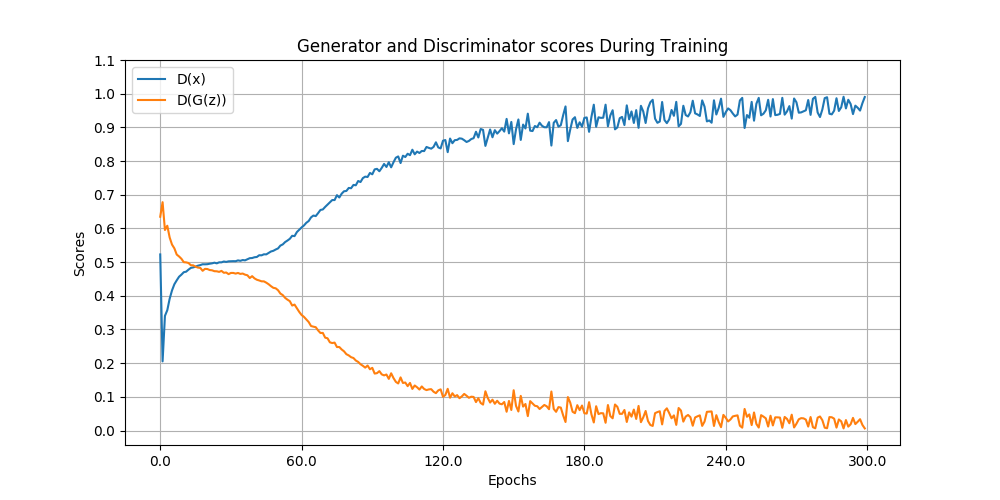
\includegraphics[width=0.9\textwidth]{Figures/LossG_et_Convergeance/scores300-64.png}
    \caption{Moyenne des réponse de \(D\) pour les images réels en bleu et les images générées en orange, au cour de l'entraînement.}
    \label{fig:fig5}
\end{figure}

\begin{figure}[!h]
    \centering
    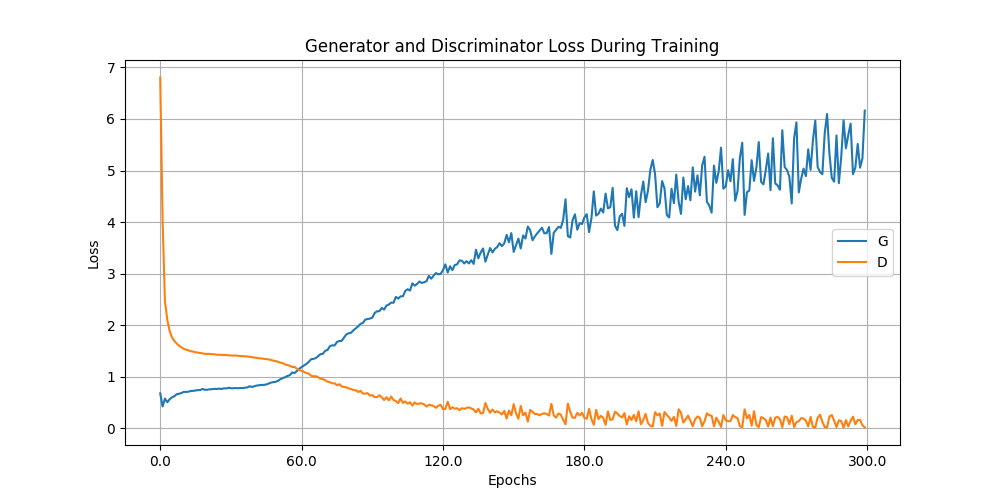
\includegraphics[width=0.9\textwidth]{Figures/LossG_et_Convergeance/losses300-64.png}
    \caption{Valeurs des fonction de pertes de \(G\) (en bleu) et \(D\) (en orange), au cour de l'entraînement.}
    \label{fig:fig6}
\end{figure}

\begin{figure}[t]
    \centering
    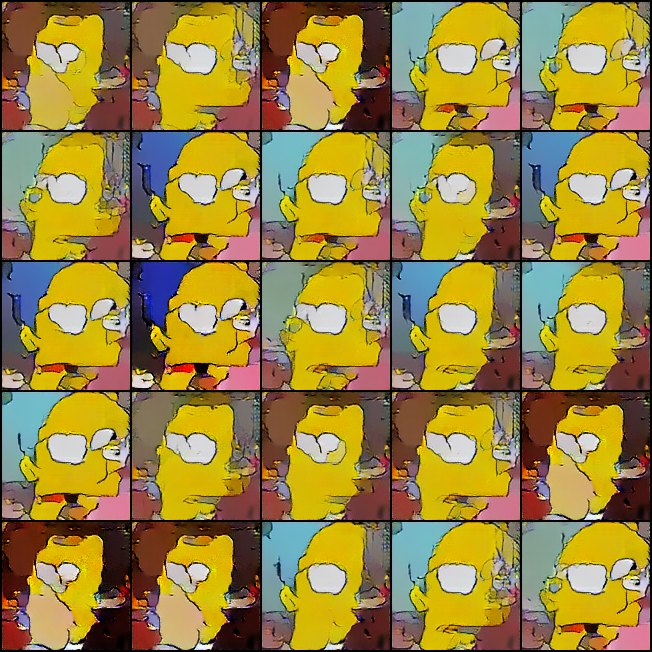
\includegraphics[width=0.5\textwidth]{Figures/LossG_et_Convergeance/collapse_980.png}
    \caption{Exemples d'images générer lors du collapse d'un générateur. On constate une faible diversité ainsi qu'une incohérences des images par rapport au dataset.}
    \label{fig:fig7}
\end{figure}

\subsection{Comparaison des espaces latent connu et générer}
\label{sec:ComparaisonLS}
Vous pouvez voir sur la figure x des images extraite du dataset FDD.
Après avoir entraîner et paramétrer différents modèles a générer des images cohérentes par rapport a celles du dataset nous avons pu générer les images visible dans les figures x. 
En comparant ces images avec la figure x on ne constate aucune correspondance entre celles générer par G et celles construite en utilisant les formules Fractal Dream \ref{sec:FDD}.
Ce résultats tendes a montrer que l'espace latent de G n'a pas développer de correspondance avec l'espace des paramètres de FDD durant sont entraînement. 

\begin{figure}[!h]
    \centering
    \begin{subfigure}[b]{0.32\textwidth}
        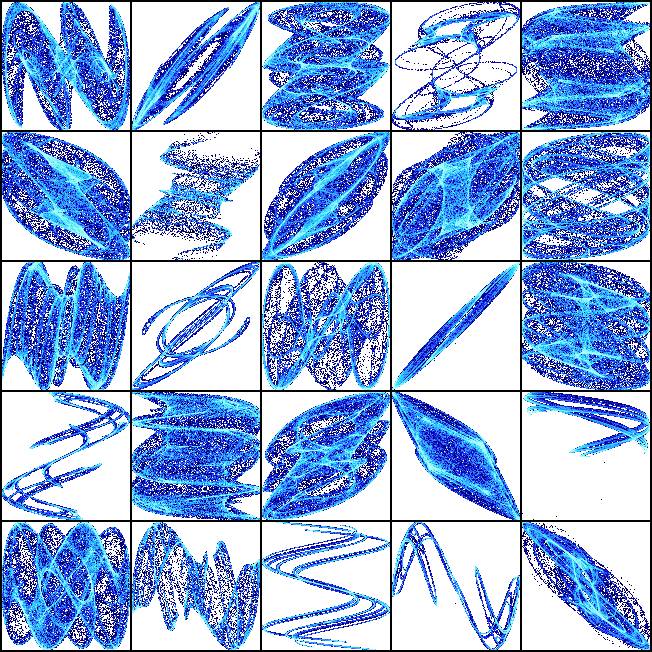
\includegraphics[width=\textwidth]{Figures/ComparaisonLS/dataset_sample.png}
        \caption{Des éléments extrait du dataset Fractal Dream Dataset.}
    \end{subfigure}
    \begin{subfigure}[b]{0.32\textwidth}
        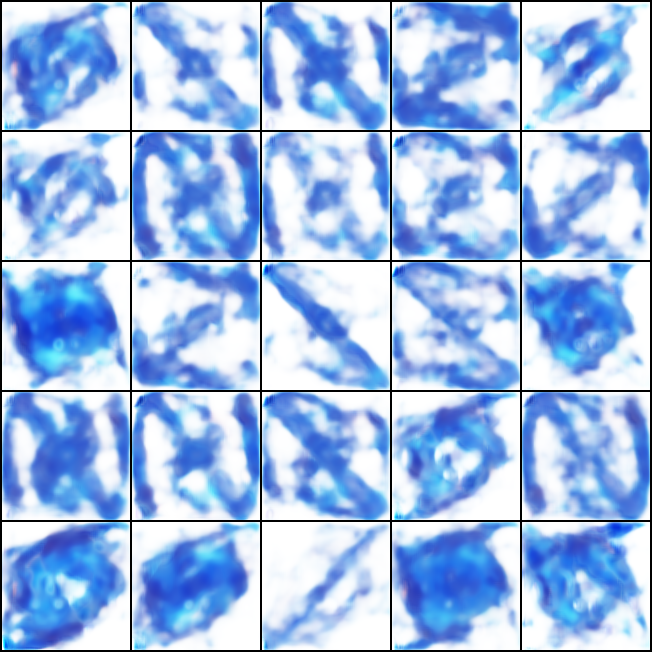
\includegraphics[width=\textwidth]{Figures/ComparaisonLS/scan7_eps0,1_lrelu0,01_0.png}
        \caption{Des images générer par un générateur entraîner par un AAE.}
    \end{subfigure}
    \begin{subfigure}[b]{0.32\textwidth}
        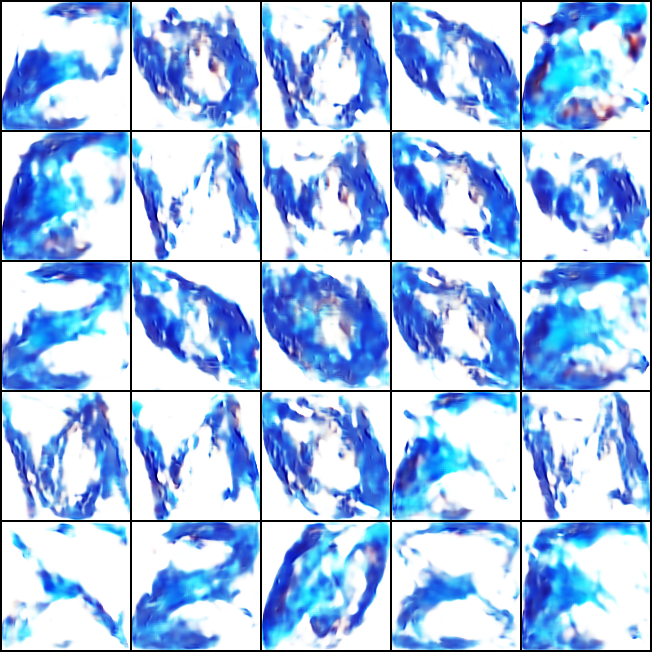
\includegraphics[width=\textwidth]{Figures/ComparaisonLS/scan8_eps0,1_lrelu1e06_0.png}
        \caption{Des images générer par un autre générateur entraîner par un AAE.}
    \end{subfigure}
    \caption{Les images générer l'on était en utilisant un vecteur latent correspondant au paramètres utiliser pour calculer les images extraite du dataset visible a droite.}
    \label{fig:fig8}
\end{figure}
%\subsection{Interpolation dans l'espace latent}

%%%%%%%%%%%%%%%%%%%%%%%%%%%%%
\section{Conclusions et perspectives}
\label{sec:Conclusion}

\subsection{Apprentissage des GANs}
L'apprentissage des GANs est une tâche ardue et nous avons eu besoin de beaucoup de test avant d'arriver a un résultats un tant soit peu convaincant. Le grand nombre d'hyper-paramètres ainsi que les vides théoriques présenter section \ref{sec:CompEtLimites} pose de nombreuse difficultés. Néant moins les résultats obtenus, avec les Simpsons notamment sont tout a fait convaincant.

\subsection{Découverte et prise en mains de nombreux outils}
Durant le stage j'ai était amener à me former a de nombreuse technologies et outils.
On peut cité parmi les plus importants Pytorch \cite{paszke2017automatic} ou encore Tensorboard \cite{tensorflow2015-whitepaper}, a ceci s'ajoute également un usage quotidien de Linux et de Python qui mon permis de découvrir de nombreux logiciels et bibliothèques.
Ensemble ces outils s'agrège a ceux étudier lors de mon Master et me permettront, je l'espère, de commencer ma vie professionnel sure de bonnes bases.

\subsection{Premier pas dans le monde professionnels}
Les laboratoires de recherche sont un monde particuliers que j'avais déjà pu approcher lors de mes études, ce stage ma permis de les découvrir en détails. J'ai pu apprendre tout ce qui fait le monde professionnel : horaires fixes, journée complètes, réunions de travail ect...
Ces nouvelles expériences forme le début de mon parcours professionnel.

\newpage
%{\bf Appendices}: Appendices, if any, directly follow the text and the references (but see above).  Letter them in sequence and provide an informative title: {\bf Appendix A. Title of Appendix}.
%\section*{Acknowledgements}

%The acknowledgements should go immediately before the references.  Do
%not number the acknowledgements section. Do not include this section
%when submitting your paper for review.

\section*{Remerciements}
Je tiens à remercier Laurent Perrinet pour m'avoir encadrés et guidés durant ce Stage.

\bibliography{biblio}
\bibliographystyle{acl}
%%%%%%%%%%%%%%%%%%%%%%%%%%%%
\newpage

\section{Annexes}
\begin{appendix}
\section{-  Formule des Fractal Dream}
\label{appendix:annexe1}
La formule ci-dessous permet de calculer le point suivant d'un attracteur de type Fractal Dream a partir des coordonnées du point actuel et de 4 paramètre données.
En utilisant cette formule successivement un grand nombre de fois on peut calculer l'image correspondant a l'attracteur pour des paramètres et un point de départ choisi.  

    \begin{table}[hb]
      \begin{tabular}{l}
      \hline
      Algorithme 3: Calcul du point suivant d'un Fractal Dream\tabularnewline
      \hline
      Entrées: \((x, y)\) coordonnées du point courant, \((a, b, c, d)\) paramètres de l'attracteur \tabularnewline
      Sortie: \((x', y')\) les coordonnées du point suivant\tabularnewline
      \hline
      \(x' \leftarrow sin(y*b)+c*sin(x*b)\)\tabularnewline
      \(y' \leftarrow sin(x*a)+d*sin(y*a)\)\tabularnewline
      \tabularnewline
      return \((x', y')\);\tabularnewline
      \hline
      \end{tabular}
      \label{tab:tab3}
    \end{table}
    
Pour l'exemple les paramètres utiliser pour générer les trois images de la figure \ref{fig:fig2} sont respectivement :\\
 1 : \(x = -0,00545687187361743 ~y = -0,5312304575586382 ~a = 1,8197494653032407 ~b = 2,422111729355857 ~c = 1,4944898296889655 ~d = 2,487490210145214\)\\
 2 : \( ~x = -0,319459804135373 ~y = -0,0981842500805612 ~a = 0,42291442353441633 ~b = 1,7253282321258185 ~c = 1,4272325555244099 ~d = 1,3701336149016234\)\\
 3 :  \(~x = -0,9333646250089 ~y = -0,3698044331245828 ~a = -1,9514116449042127 ~b = -0,376713271698188 ~c = -1,1759178511809651 ~d = -1,7157801385982319\)

\end{appendix}

%%%%%%%%%%%%%%%%%%%%%%%%%%%%


\end{document}
